%!TEX root = ../08-Interference.tex
\chapter{Newton's Rings}

The curvature radius of a biconvex lens and the refractive index of water are determined by analyzing the lense's Newton's rings interference pattern.

\section{Setup}

Newton's rings are an interference phenomena that occurs when a transparent spherical object is placed on a flat reflective surface and is illuminated from the top with monochromatic, coherent light.
A series of concentric rings can be observed.

A portion of the incident light is reflected when exiting the lens, the light \todo{bla bla bla}
The two beams have a path difference of $2 d$, additionally a phase inversion occurs at the substrate, where the light enters a more optically dense medium.

\todo{math: he didn't do his}

A microscope slide is used as the substrate.
The lens and substrate are placed in a microscope with a XY-stage and a vernier scale on both axes.
The rings are centered around the crosshair.
A crosshair is used to center edges of the rings along one axis, the rings' radii are read on the vernier scale.

\begin{figure}
	\centering
	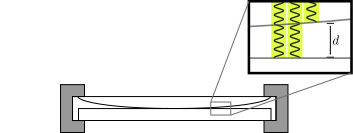
\includegraphics[width=.6\textwidth]{img/newtons-rings.pdf}
	\caption{Newton's rings}
	\caption*{based on \url{https://en.wikipedia.org/wiki/Newton\%27s_rings\#/media/File:Newton\%27s_rings_02.svg}}
\end{figure}

\section{Evaluation}
